\chapter{Current Feedback}
\section{Overview}
\label{sec:overview_motor}
The key focus of this section is the discussion of adding a current feedback sub-system to the autonomous `mouse', addressing the limitation that does not allow for motor current sensing, meaning deteriorating battery health and current spikes during hill ascent cannot be considered when controlling motor speed. The section suggests altering the motor drive sub-system of the `mouse' to add motor current feedback. The motor drive sub-system currently varies the voltage across a \(6\) V DC motor \cite{mfa_motor} using a MOSFET or BJT acting as an electronic switch, toggling on and off with a PWM control signal \cite{Robinson2025}. The proposed solutions must provide reliable, accurate current readings and not adversely affect motor drive control. The solutions will be evaluated based on their stability, simplicity of integration and cost of implementation.

\section{Design Concepts and Methods}
\subsubsection{Shunt Resistor}
\begin{wrapfigure}{r}{0.4\textwidth}
  \begin{center}
    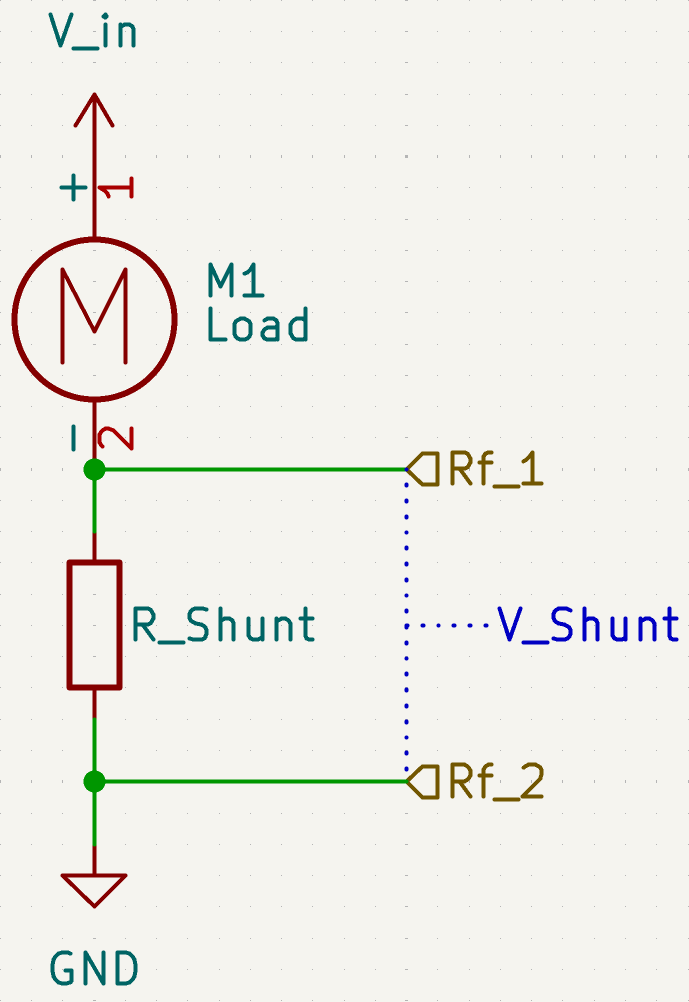
\includegraphics[width=1\linewidth]{circuits/shun_res_theory.png}
  \end{center}
  \caption{Shunt Resistor Circuit with a motor as circuit load.}
  \label{fig:shunt_theory}
\end{wrapfigure}

Designs F and G utilise a shunt resistor to measure the current within the motor. Generally, a shunt resistor is a precision low-resistance device connected in series with the load (Fig.\ref{fig:shunt_theory}), ensuring that the load current flows through it and generating a voltage directly related to the magnitude of the current as per Ohm's Law:

\begin{equation}
    V=IR
    \label{equ:Ohms_law}
\end{equation}

The potential difference (voltage drop) is measured across the terminals of the shunt resistor. Rearanging equation \ref{equ:Ohms_law} for \(I\) in terms of \(V\) and \(R\) (Equation \ref{equ:Ohms_law_current}), you can calculate the current from the known resistance and measured voltage.
\begin{equation}
    I=\frac{V}{R}
    \label{equ:Ohms_law_current}
\end{equation}

Shunt resistor values are commonly in the milliohm range to suit different current sensing applications. By choosing a smaller resistance the voltage drop across the shunt resistor will be smaller, and reducing the voltage drop into the millivolt range can minimise power loss and circuit disruption.  The small voltage developed is commonly amplified to improve signal accuracy before further processing.


\subsection{Design F: Low-Side Motor Drive}
\label{sec:low_motor}
\begin{wrapfigure}{r}{0.5\textwidth}
  \begin{center}
    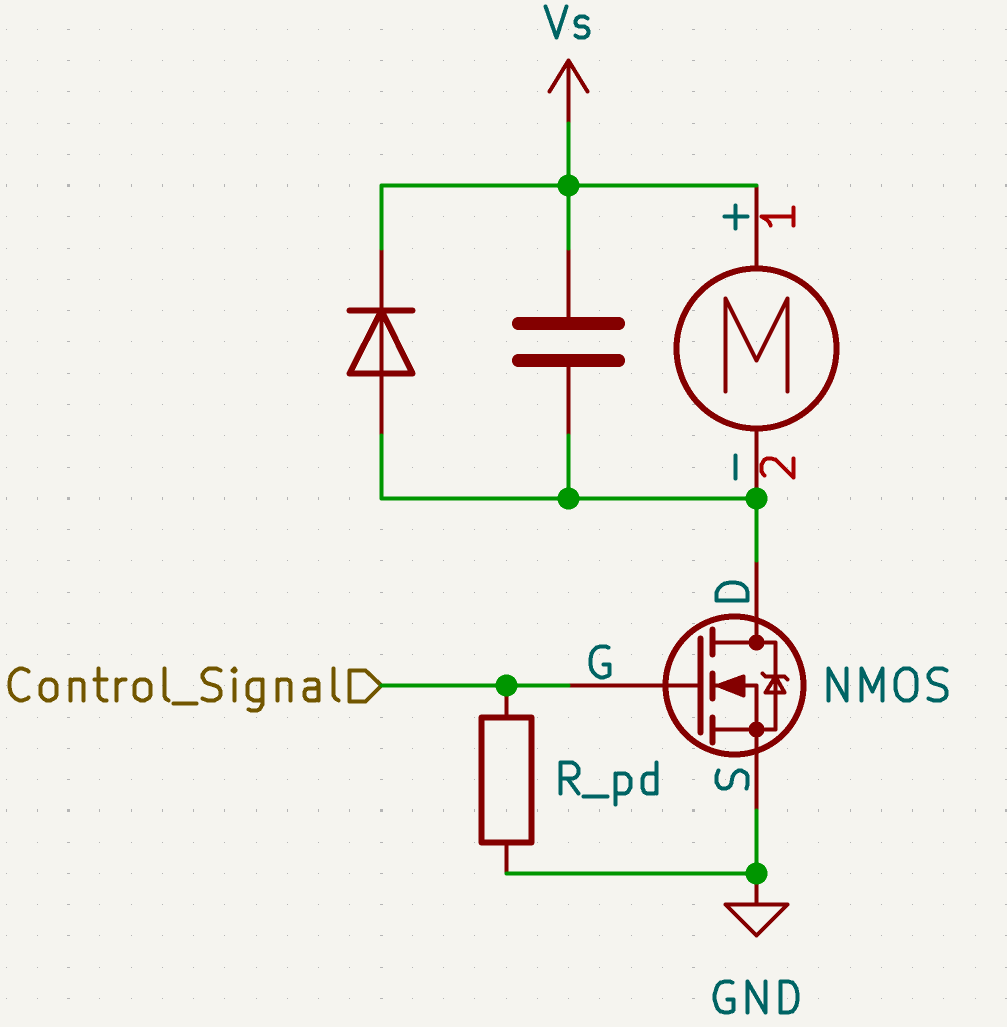
\includegraphics[width=1\linewidth]{circuits/low_side_mos.png}
  \end{center}
  \caption[Low-side N-channel MOSFET Motor Drive Circuit]{Low-side N-Channel MOSFET drive circuit controlling a DC Motor Load with transient suppression components.}
  \label{fig:low_drive_theory}
\end{wrapfigure}

Design F used a low-side N-channel MOSFET drive circuit (Fig.\ref{fig:low_drive_theory}) to control the operation of a DC motor. The MOSFET acts as an electronic switch in this configuration, enabling or disabling current flow through the motor. When acting like a switch the N-channel MOSFET must have a gate-source voltage (\(V_{GS}\)), defined as \(V_{GS}=V_G-V_S\), sufficiently above the threshold voltage (\(V_{t}\)) potential for reliable conduction \cite[p.297]{Sedra_Smith_Microelectronic}. The gate voltage (\(V_{G}\)) is supplied by a control signal applied to the gate terminal (`Control\_Signal'), and the source voltage (\(V_s\)) is set to GND.

Varying the duty cycle of the control signal modulates the average voltage and current supplied to the motor, providing adjustable speed control. When the signal is high the MOSFET conducts and the inverse is true when the circuit is low. The voltage observed can be calculated using equation \ref{equ:pwm_volt} as described by Rashid \cite[p. 920]{Muhammad_PowerElectronics}; where \(v\) is the voltage observed, \(V_{s}\) is the supply voltage and \(\delta\) is the normalised duty cycle (\(0\rightarrow1.0\)).

\begin{equation}
    v = \delta V_{s}
    \label{equ:pwm_volt}
\end{equation}
\vspace{1em}

Furthermore, a pull-down resistor (`R\_pd') is utilised within the circuit connecting the gate and source of the transistor; this prevents the gate voltage from floating and pulls it to the same potential (GND) when the signal is low, closing the MOSFET switch.

In addition, as DC motors are inductive loads, switching them introduces transient voltage spikes. The voltage spikes are particularly obvious during turn-off events. To address the voltage spikes and increase stability it is common practice to add:

\begin{itemize}
    \item A flyback diode is placed directly across the motor terminals \cite[pp.970-971]{Muhammad_PowerElectronics}, with its cathode connected to the top of the motor. This provides a path for the inductive current from the motor when the MOSFET switches off, safely clamping the voltage spike and protecting the MOSFET from overvoltage conditions.
    \item A snubber capacitor is placed across the motor terminals \cite[p.380]{Williams_EMC} to suppress high-frequency voltage transients and reduce EMI generated by the DC motor.
\end{itemize}


\subsection{Design G: High-Side Motor Drive}
\label{sec:highside}
\begin{figure}[H]
    \centering
    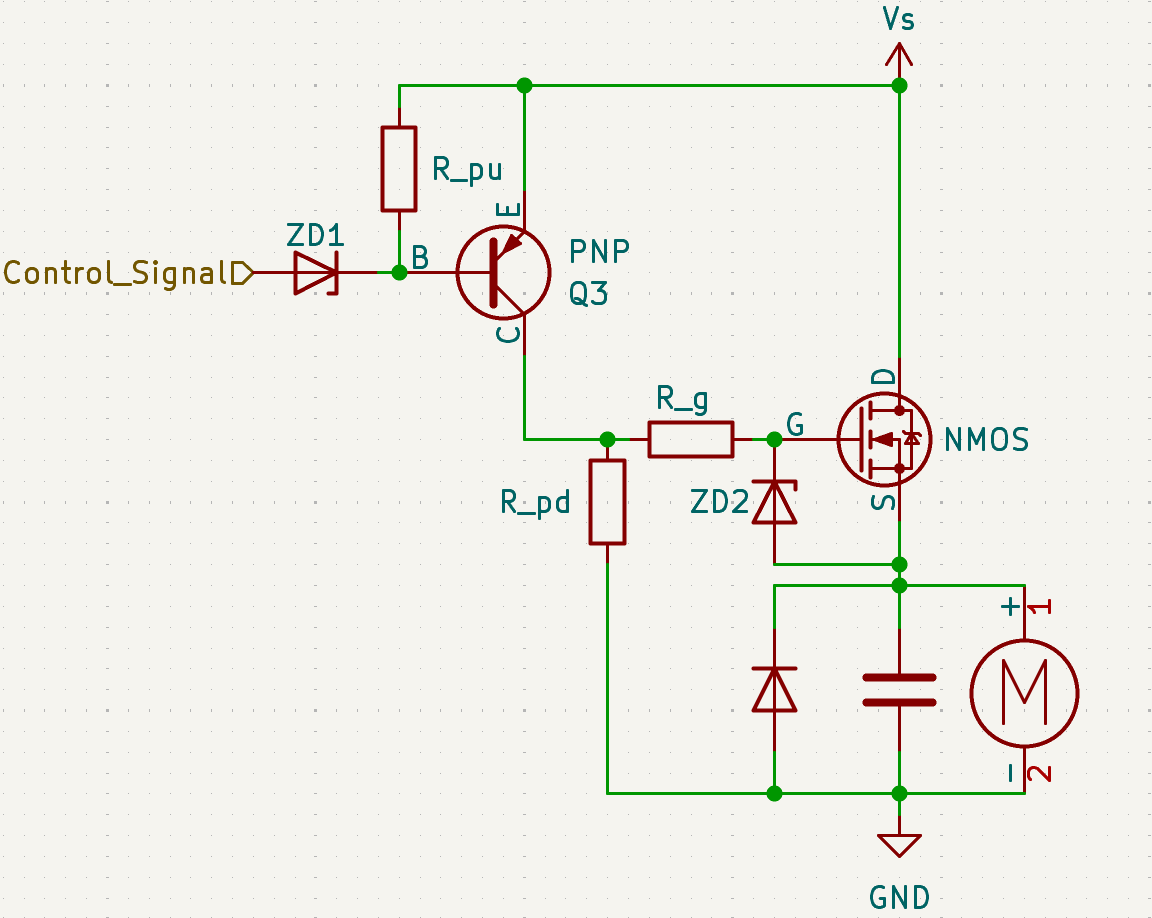
\includegraphics[width=1\linewidth]{circuits/high_side_mos.png}
    \caption[High-side N-channel MOSFET Motor Drive Circuit]{Schematic of a High-side N-channel MOSFET motor drive circuit with PNP transistor level-shifting stage. Controlling a DC motor with transient suppression components.}
    \label{fig:high_drive_theory}
\end{figure}

Design G used a high-side N-channel MOSFET drive circuit (Fig.\ref{fig:high_drive_theory}) to control the operation of a DC motor. Using a high-side switch allows the load to be directly connected to GND. However, driving an N-channel MOSFET in a high-side position presents a challenge, as the gate-source voltage (\(V_{GS}\)) must be raised sufficiently to turn the device on and in a high-side position when conducting the source is connected to the voltage supply (\(V_s\)).

A PNP transistor level-shifting stage is employed to overcome this, shifting the input control signal to the \(V_s\) level, enabling a low-voltage logic-level control signal to switch the high-side N-channel MOSFET. A PNP transistor works by allowing a current to flow from the emitter to the collector when there is sufficient current observed from the emitter to base (forward-bias) \cite[p.246]{Sedra_Smith_Microelectronic}.

The control signal (`Control\_Signal') is applied to the PNP base via a series-connected zener diode (`ZD2'). Adding a zener diode provides overvoltage protection, ensuring that the PNP transistor’s base-emitter junction remains within its safe operating limits. A pull-up resistor (`R\_pu') is connected between the PNP transistor’s base and the positive supply rail, keeping the transistor turned off when the control signal is floating or at a logic-high level. When the signal transitions low, the base-emitter junction of the PNP transistor becomes forward-biased, turning the transistor on. This action connects the emitter to the collector, allowing the positive supply rail to connect to the N-Channel MOSFET’s gate terminal via a gate resistor (`R\_g'). As previously discussed in Section \ref{sec:low_motor}, as the gate voltage rises it exceeds the MOSFET’s source potential (at the same potential as the supply rail \(`V_s\) during conduction), allowing current to flow from the drain to the source pin and hence through the motor load to GND.

The gate resistor performs two key tasks within this circuit, primarily limiting the current into the gate terminal, which controls the transistor's switching speed. Additionally, the resistor protects the PNP transistor from transient currents observed during transistor switching events. Typically, gate resistor values are between \(1\rightarrow100\Omega\) when used in a motor drive circuit. To further improve system robustness, a zener diode (`ZD2') is placed across the MOSFET’s gate and source terminals. The zener clamps the gate voltage (\(V_G\)) to a safe maximum value, protecting the MOSFET from overvoltage conditions.

The motor load circuit and pull-down resistor (`R\_pd') are included as per the details outlined in Section \ref{sec:low_motor}, the main difference being that the motor load now connects to the MOSFET source pin and GND.

It should be noted that with this design, the PWM response is inverted. When the PWM control signal is low the N-Channel MOSFET is conducting the inverse is true when the signal is high.

\section{Procedures}
\subsection{Design F: Low-Side Motor Drive}
\label{sec:low_side_motor}
\label{sec:6}
\subsubsection{Assembly}
\begin{figure}[H]
    \centering
    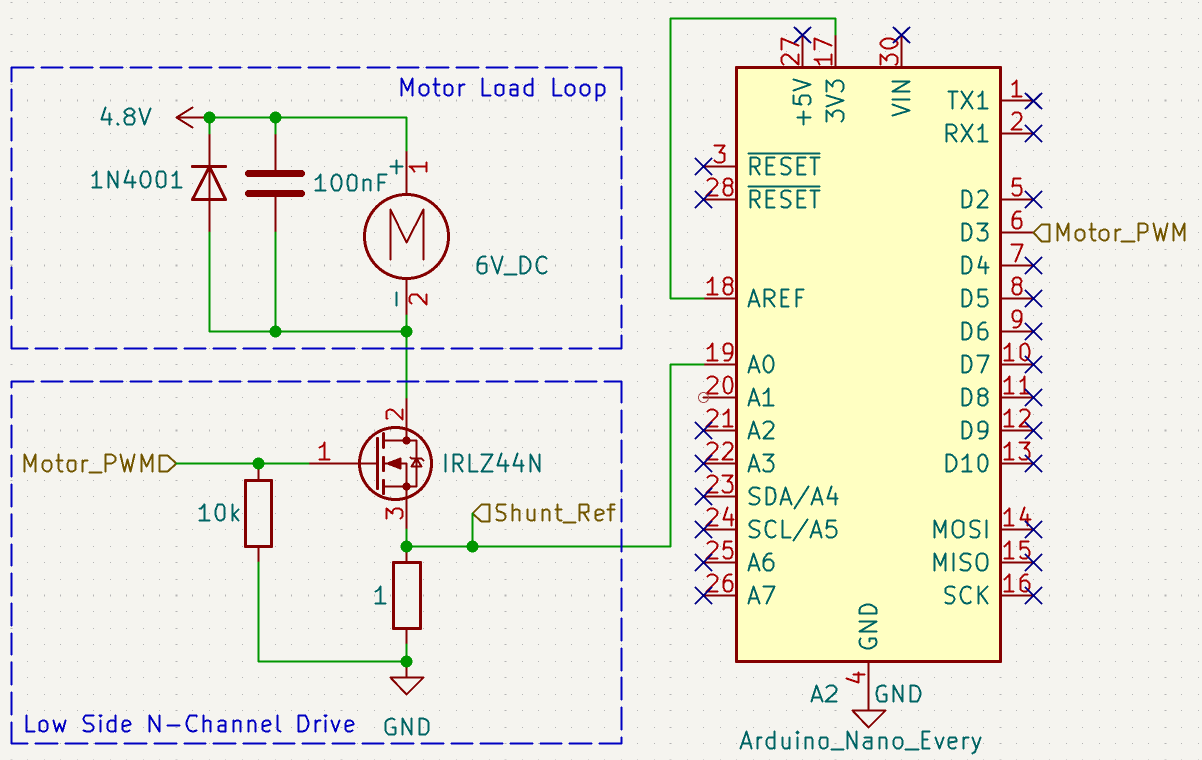
\includegraphics[width=1\linewidth]{circuits/current_low.png}
    \caption[Design F: Schematic]{Schematic diagram of Design F; a Low-side motor drive circuit with current sensing shunt resistor.}
    \label{fig:low_current_circuit}
\end{figure}

Design F was built on a standard RH-32 breadboard following the design outline in Figure \ref{fig:low_current_circuit}. Firstly, the N-Channel drive circuit was assembled using an IRLZ44N N-Channel MOSFET \cite{Infineon_IRLZ44N}; the source (pin 3) of the MOSFET was connected to the \(1\) \(\Omega\)  current sensing shunt resistor in series to GND and the gate (pin 1) is connected to the GND with a \(10\) k\(\Omega\) pull-down resistor. The IRLZ44N was choosen for its logic level of \(3.3\) V (Matches Arduino PWM \cite{Microchip_ATmega4809}) and previous use in the `mouse' race as a MOSFET switch.

Secondly, the motor load loop was assembled using a motor from a mouse chassis. First, the motor was connected to the breadboard with single-core wires. Following on, a 1N4001 \cite{Kitronik_1N4001} flyback diode and \(100\) nF snubbing capacitor were connected over the motor as seen in Figure \ref{fig:low_current_circuit}. Care was taken in orienting the 1N4001 making sure the anode was connected to the top of the motor. After that the \(4.8\) V DC 3631A lab power supply rail was connected to the top side of the motor.

Third, the Arduino Nano Every \cite{Arduino_Every} was placed into the breadboard over the central channel. The analogue pin was connected first with A0 connecting to the node between the MOSFET and resistor (Shunt\_Ref). The D3 pin (Motor\_PWM) was then connected to the gate of IRLZ44N. Following on, the GND was connected to the Arduino and the \(3.3\) V DC supply rail from the Arduino was connected to the analogue reference (AREF) pin of the Arduino. By setting the AREF at \(3.3\) V DC the ADC within the Arduino Nano could measure at increments of \(\approx3.2\) mV (LSB) with an accuracy of \(\pm0.5\)LSB \cite{Microchip_ATmega4809}. 

Finally, an Arduino program was developed and uploaded to the Arduino Nano Every (Appendix \ref{app:Arduino} Listing \ref{cod:current_1ref}). The program controlled the speed of the DC motor via Pulse Width Modulation (PWM) and monitored the current drawn by the motor. The PWM duty cycle was adjusted within the code to set the motor’s operating speed. The current was measured using one reference point (`Shunt\_Ref') achieved through the analogue input pin A0. The potential difference between the reference point and GND was recorded, and the value was then stored in an array. A moving average algorithm was implemented within the program and calculated based on the array values. The average calculated value was then converted into a current using equation \ref{equ:Ohms_law_current}, as the resistance was \(1\Omega\) the value was directly converted from voltage to current. This value was multiplied by a constant of \(0.0032\) (\(3.3V/1024\approx0.0032\))to convert from the digital signal to an analogue value. This approach allowed for a smoother, more representative current value for each operating condition. The processed current data was then output via the Arduino’s serial interface. 

\subsubsection{Testing}
The steps for Testing Design F are as follows:

\begin{enumerate}
    \item Design F power supply rails and circuit GND were verified using a KeySight 34450A multimeter.
    \item The `Motor\_PWM' was varied from \(0\rightarrow128\) incrementing in values of 8, representing a duty cycle range \(0\rightarrow50\%\). The motor voltage and current were measured thrice at each PWM value using a KeySight 34450A multimeter. The voltage values were recorded in Excel and compared to the expected voltages. In addition, the motor current values were recorded in Excel along with the Arduino calculated current values seen on the Serial Monitor.  
    \item More current readings were then taken from the motor and Arduino whilst applying slight resistance to the wheel, whilst the `Motor\_PWM' was varied from \(0\rightarrow128\) incrementing approximating to a 10\% change in duty cycle, recording values in Excel.
\end{enumerate}

During testing, it was noted that the voltage readings over the motor seemed to be off expectations (Appendix \ref{app:data} Table 5). Waveform's on the oscilloscope suggested the back EMF voltage from the motor seriously impacted readings (Appendix \ref{app:data} Figure \ref{fig:osc_emf}). A secondary test was completed, replacing the motor load loop with a \(1\) k\(\Omega\) resistor connected to the \(4.8\) V DC 3631A lab power supply rail and pin 2 (Drain) of IRLZ44N. The `Motor\_PWM' was varied \(0\rightarrow128\) incrementing in values approximating to a 10\% change in duty cycle. The voltage across its terminals was then measured using the KeySight 34450A multimeter, recording values in Excel. 

All measurements were taken after a 5-second stabilisation period to minimise transient effects and were conducted at room temperature (approximately 22°C). The multimeter readings were tabulated, and statistical analysis was performed to evaluate the motor's PWM response and the absolute error for the current readings.



\subsection{Design G: High-Side Motor Drive}
\label{sec:7}
\subsubsection{Assembly}

\begin{figure}[H]
\centering
    \centering
    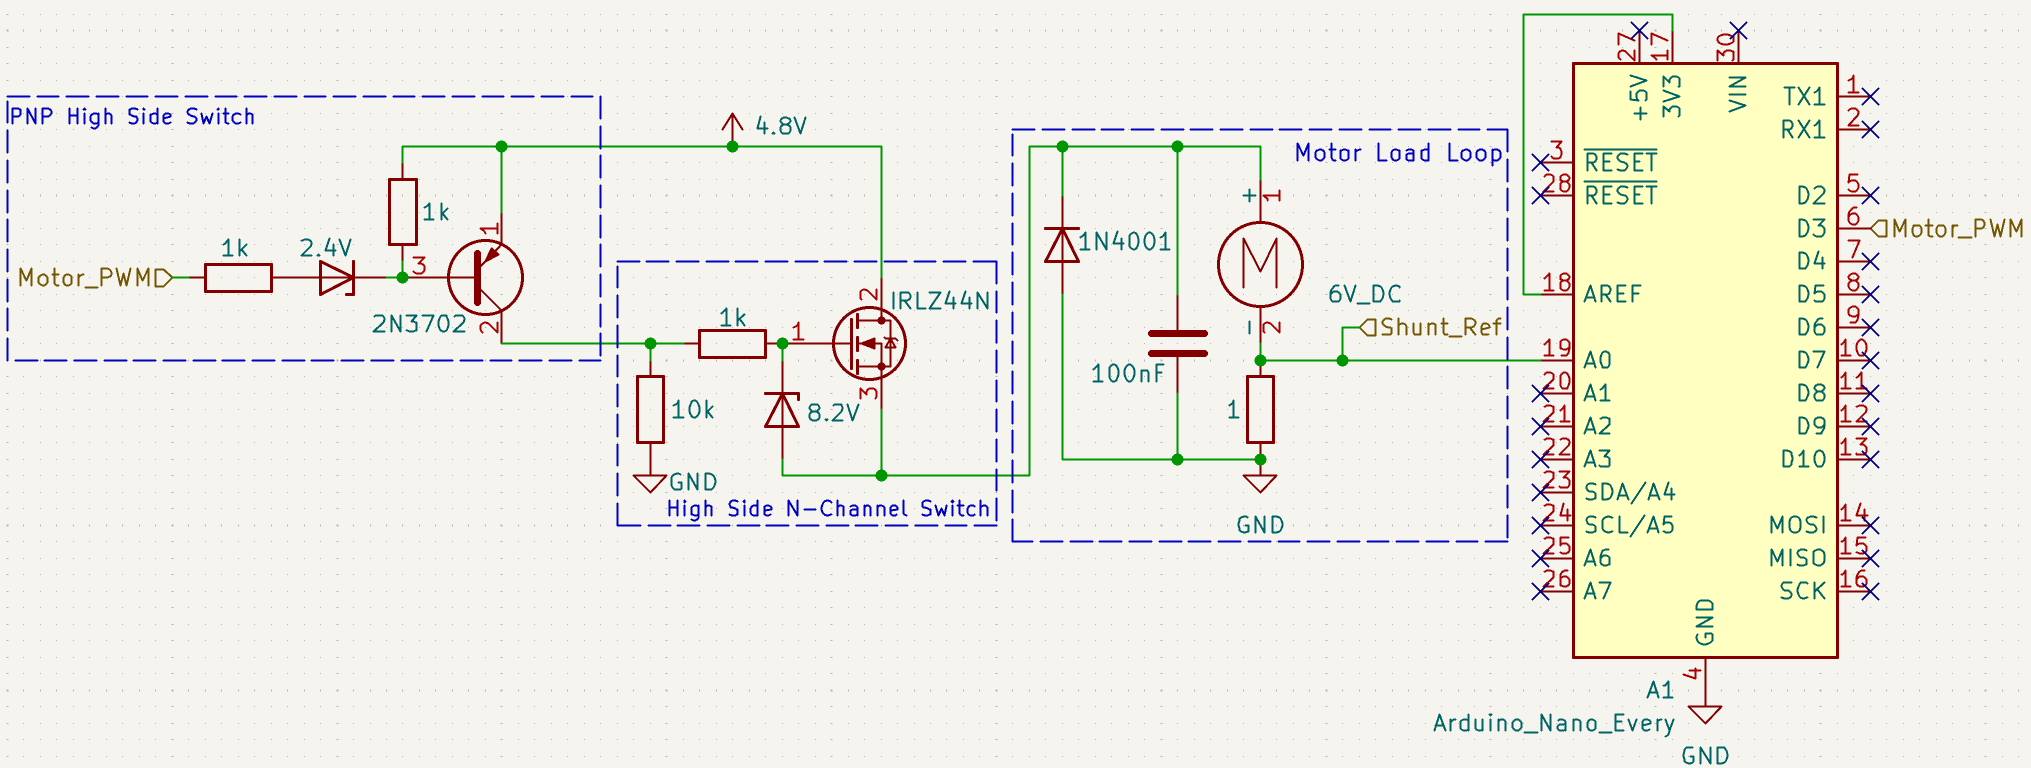
\includegraphics[width=1\linewidth]{circuits/motor_control.png}
    \caption[Design G: Schematic]{Schematic diagram of Design G; a High-side motor drive circuit with current sensing shunt resistor.}
\label{fig:high_side_motor}
\end{figure}

Design F was built on a standard RH-32 breadboard following the schematic in Fig.\ref{fig:high_side_motor}. Firstly, the PNP high side switch was assembled using a 2N3702 \cite{Components101_2N3702}; the emitter (pin 1) of the PNP transitor was connected to the \(4.8\) V DC supply rail,  a \(1\) k\(\Omega\) resistor was connected between the base (pin 3) of the transistor and the \(4.8\) V DC 3631A lab power supply rail. Next, the base clamping \(2.4\) V zener diode was connected with the cathode connecting to the 2N3702 base (pin 3) and on the anode was connected to a \(1\) k\(\Omega\) current limiting resistor.

Secondly, the high-side N-Channel switch was built (Fig.\ref{fig:high_side_motor}) utilising an IRLZ44N N-Channel MOSFET \cite{Infineon_IRLZ44N}; the gate (pin 1) was connected with a \(1\) k\(\Omega\) gate resitor to the collector of IRLZ44N (pin 2) and the drain (pin 2) was connected to the \(4.8\) V DC 3631A lab power supply rail. A gate clamping \(8.2\) V zener diode was connected with the anode connecting to the IRLZ44N source (pin 3) and the cathode directly to the gate. As the schematic shows, a final \(10\) k\(\Omega\) pull-down resistor was connected to GND.

Third, the motor loop circuit (Fig.\ref{fig:high_side_motor}) was assembled as previously described in section \ref{sec:low_side_motor}, with the following variations:
\begin{itemize}
    \item The current sensing shunt resistor was connected to the bottom of the motor, then to ground.
    \item The anode of the flyback diode and the capacitor were connected to GND instead of the drain of IRLZ44N.
    \item The top side of the motor was connected to the source of IRLZ44N and not to the \(4.8\) V DC supply rail.
\end{itemize}

Fourth, the Arduino Nano Every was placed into the breadboard over the central channel. The analogue pin was connected first with A0 connecting to the shunt resistor and motor node (`Shunt\_Ref'). The D3 pin (Motor\_PWM) was then connected to the current limiting resistor for the base of 2N3072 as seen in Fig.\ref{fig:high_side_motor}. Following on, the GND was connected to the Arduino and the \(+3.3\) V DC supply rail from the Arduino was connected to the analogue reference (AREF) pin of the Arduino.

Finally, the Arduino program designed for Design G (Appendix \ref{app:Arduino} Listing \ref{cod:current_1ref}) was reuploaded to the Arduino Nano Every.


\subsubsection{Testing}
The testing method for Design F followed the same procedure as outlined in Section \ref{sec:low_side_motor} including the secondary investigation, with the exception of varying the PWM from \(255\rightarrow128\), representing a duty cycle range of \(100\rightarrow50\%\). All measurements were taken under the same conditions and analysed accordingly as defined in \ref{sec:low_side_motor}.

\section{Results}
\subsection{Design F: Low-Side Motor Drive}

\begin{table}[H]
    \centering
    \caption[Design F: Current Measurements]{Design F measured current compared to Arduino current calculated values (Appendix \ref{app:data} Table \hyperref[tab:A.8]{A.8})}
    \label{tab:Low_current}
    \begin{tabular}{|c|c||c|c||c|}\hline
     &&\multicolumn{2}{|c||}{Current (A)} &  \\\hline
    PWM &Duty Cycle \%&Multi-meter Average&Arduino Average&Absolute Error \\ \hline 
    0 &0&0.001&0.00&-0.001\\ \hline
    8 &3.14&0.014&0.01&-0.004\\\hline
    16 &6.27&0.043&0.04&-0.003\\\hline
    24 &9.41&0.080&0.08&0.000\\\hline
    32 &12.55&0.113&0.12&0.007\\\hline
    40 &15.69&0.125&0.13&0.005\\\hline
    48 &18.82& 0.163& 0.16& -0.003\\\hline
    56 &21.96& 0.171& 0.17& -0.001\\\hline
    64 &25.1& 0.184& 0.18& -0.004\\\hline
    72 &28.24& 0.188& 0.19& 0.002\\\hline
    80 &31.37& 0.200& 0.20& 0.000\\\hline
    88 &34.51& 0.211& 0.21& -0.001\\\hline
    96 &37.65& 0.221& 0.22& -0.001\\\hline
    104 &40.78& 0.221& 0.21& -0.011\\\hline
    112 &43.92& 0.208& 0.21& 0.002\\\hline
    120 &47.06& 0.214& 0.22& 0.006\\\hline
    128 &50.2& 0.220& 0.22& 0.000\\\hline\end{tabular}  
\end{table}

\begin{table}[H]
    \centering
    \caption[Design F: Current Measurements]{Design F measured current compared to Arduino current calculated values with pressure applied to wheel (Appendix \ref{app:data} Table \hyperref[tab:A.9]{A.9})}
    \label{tab:Low_current_pressure}
    \begin{tabular}{|c|c||c|c||c|}\hline
     &&\multicolumn{2}{|c||}{Current (A)} &  \\\hline
    PWM &Duty Cycle \%&Multi-meter Average&Arduino Average&Absolute Error \\ \hline 
    24 &9.41&0.085&0.09&0.005\\ \hline
    56 &21.96&0.313&0.32&0.007\\\hline
    80 &31.37&0.508&0.51&0.002\\\hline
    104 &40.78&0.710&0.71&0.000\\\hline
    128 &50.2&0.992&0.99&-0.002\\\hline\end{tabular}  
\end{table}

The observed Arduino current values closely followed the multi-meter values (Tables \ref{tab:Low_current}, \ref{tab:Low_current_pressure}).

\begin{table}[H]
    \centering
    \caption[Design F: Voltage Measurements \(1\) k\(\Omega\) Resistor Load]{Design F measured voltage when the circuit load is a \(1\) k\(\Omega\) resistor (Appendix \ref{app:data} Table \hyperref[tab:A.10]{A.10}).}
    \label{tab:low_voltage_1k}
    \begin{tabular}{|c|c||c|c||c|}\hline
     &&\multicolumn{2}{|c||}{Voltage (V)} &  \\\hline
    PWM &Duty Cycle \%&Expected&Multi-meter Average&Absolute Error \\ \hline 
    0&0&0&0.000&0.000\\ \hline
    24&9.41&0.45&0.200&0.251\\\hline
    56&21.96&1.05&1.057&-0.003\\\hline
    80&31.37&1.51&1.500&0.006\\\hline
    104&40.78&1.96&1.958&-0.001\\\hline
 128& 50.2& 2.41& 2.410&0.000\\\hline\end{tabular}  
\end{table}

In Table \ref{tab:low_voltage_1k} the discrepancy between expected voltage and measured voltage at 9.4\% duty cycle may be caused by incorrect multi-meter averaging of short pulses. However, with the remaining data the measured and expected values closely agree.

\subsubsection{Cost of Implementation}

\begin{table}[H]
\centering
\caption{Alphabetically Ordered Estimated Component Costs for Design F}
\begin{tabular}{|l|c|c|c|}
\hline
\textbf{Component}                & \textbf{Quantity} & \textbf{Unit Price (£)} & \textbf{Total Price (£)}\\ \hline
100nF Polyester Capacitor\cite{rs_100nfcap_poly} & 1 & 0.486 & 0.486\\ \hline
10kΩ Resistor \cite{rs_10kresistor} & 1 & 0.07 & 0.07\\ \hline
1Ω Resistor \cite{rs_res1}& 1 & 0.162 & 0.162\\ \hline
1N4001 Diode \cite{rs_1n4001} & 1 & 0.103 & 0.103\\ \hline
NiMH 1.2V AA Batteries \cite{rs_nimh} & 4 & 2.243 & 8.972\\ \hline
IRLZ44N N-Channel MOSFET \cite{rs_irlz44n} & 1 & 0.717 & 0.717\\ \hline\hline
\textbf{Total Estimated Cost} &&&\textbf{£10.51}\\ \hline
\end{tabular}
\label{tab:cost_designf}
\end{table}

Table \ref{tab:cost_designf} details the individual components required for the implementation of Design F, alongside their quantities, specifications, suppliers, and unit costs based on UK-sourced pricing at the time of writing. The cost of implementation within the `mouse' would be £12.05, adding a second version of the design without additional NiMH batteries. The cost difference between the original sub-system (Appendix \ref{app:mouseecost_og}) is +£1.57 an increase in cost of \(15\%\).
\newpage
\subsection{Design G: High-Side Motor Drive}

Please note, as mentioned in section \ref{sec:highside}, the PWM and duty cycle values are inverted.

\begin{table}[H]
    \centering
    \caption[Design G: Current Measurements]{Design G measured current compared to Arduino current calculated values (Appendix \ref{app:data} Table \hyperref[tab:A.11]{A.11})}
    \label{tab:High_current}
    \begin{tabular}{|c|c||c|c||c|}\hline
     &&\multicolumn{2}{|c||}{Current (A)} &  \\\hline
    PWM &Duty Cycle \%&Multi-meter Average&Arduino Average&Absolute Error \\ \hline 
    255 &100&0.001&0.00&-0.001\\ \hline
    247 &96.86&0.012&0.03&0.018\\\hline
    239 &93.73&0.026&0.04&0.014\\\hline
    231 &90.59&0.046&0.06&0.014\\\hline
    223 &87.45&0.069&0.09&0.021\\\hline
    215 &84.31&0.096&0.13&0.034\\\hline
    207 &81.18& 0.117& 0.17& 0.053\\\hline
    199 &78.04& 0.131& 0.14& 0.009\\\hline
    191 &74.9& 0.145& 0.18& 0.035\\\hline
    183 &71.76& 0.155& 0.18& 0.025\\\hline
    175 &68.63& 0.159& 0.18& 0.021\\\hline
    167 &65.49& 0.168& 0.20& 0.032\\\hline
    159 &62.35& 0.221& 0.18& -0.041\\\hline
    151 &59.22& 0.221& 0.19& -0.031\\\hline
    143 &56.08& 0.208& 0.21& 0.002\\\hline
    135 &52.94& 0.214& 0.19& -0.024\\\hline
    127 &49.8& 0.220& 0.22& 0.000\\\hline\end{tabular}  
\end{table}

\begin{table}[H]
    \centering
    \caption[Design G: Current Measurements]{Design G measured current compared to Arduino current calculated values with pressure applied to wheel (Appendix \ref{app:data} Table \hyperref[tab:A.12]{A.12})}
    \label{tab:High_current_pressure}
    \begin{tabular}{|c|c||c|c||c|}\hline
     &&\multicolumn{2}{|c||}{Current (A)} &  \\\hline
    PWM &Duty Cycle \%&Multi-meter Average&Arduino Average&Absolute Error \\ \hline 
    231 &90.59&0.049&0.07&0.021\\ \hline
    207 &81.18&0.131&0.20&0.069\\\hline
    183 &71.76&0.238&0.29&0.052\\\hline
    159 &62.35&0.313&0.40&0.087\\\hline
    127 &49.8&0.472&0.56&0.088\\\hline\end{tabular}  
\end{table}

The observed Arduino current values are in the same order as the multi-meter values but are not close matches (Tables \ref{tab:High_current}, \ref{tab:High_current_pressure}).

\begin{table}[H]
    \centering
    \caption[Design G: Voltage Measurements \(1\) k\(\Omega\) Resistor Load]{Design G measured voltage when the circuit load is a \(1\) k\(\Omega\) resistor (Appendix \ref{app:data} Table \hyperref[tab:A.13]{A.13}).}
    \label{tab:high_voltage_1k}
    \begin{tabular}{|c|c||c|c||c|}\hline
     &&\multicolumn{2}{|c||}{Voltage (V)} &  \\\hline
    PWM &Duty Cycle \%&Expected&Multi-meter Average&Absolute Error \\ \hline 
    255&100&0&0.000&0.000\\ \hline
    231&90.59&0.45&0.194&0.257\\\hline
    207&81.18&0.9&0.319&0.584\\\hline
    183&71.76&1.36&0.931&0.425\\\hline
    159&62.35&1.81&1.151&0.656\\\hline
 127& 49.8& 2.41& 1.534&0.876\\\hline\end{tabular}  
\end{table}

The values seen in Table \ref{tab:high_voltage_1k} demonstrate a linear relationship between PWM and multi-meter voltage. However, the values measured are significantly lower than expected, particularly at lower duty cycles.


\subsubsection{Cost of Implementation}

\begin{table}[H]
\centering
\caption{Alphabetically Ordered Estimated Component Costs for Design G}
\begin{tabular}{|l|c|c|c|}
\hline
\textbf{Component}                & \textbf{Quantity} & \textbf{Unit Price (£)} & \textbf{Total Price (£)}\\ \hline
100nF Polyester Capacitor\cite{rs_100nfcap_poly} & 1 & 0.486 & 0.486\\ \hline
10kΩ Resistor \cite{rs_10kresistor} & 1 & 0.07 & 0.07\\ \hline
1kΩ Resistor \cite{rs_1kresistor} & 1 & 0.162 & 0.486\\ \hline
1Ω Resistor \cite{rs_res1}& 1 & 0.162 & 0.162\\ \hline
1N4001 Diode \cite{rs_1n4001} & 1 & 0.103 & 0.103\\ \hline
2.4V Zener Diode \cite{rs_24vzdiode} & 1 & 0.129 & 0.129\\ \hline
8.2V Zener Diode \cite{rs_82vzdiode} & 1 & 0.117 & 0.117\\ \hline
NiMH 1.2V AA Batteries \cite{rs_nimh} & 4 & 2.243 & 8.972\\ \hline
IRLZ44N N-Channel MOSFET \cite{rs_irlz44n} & 1 & 0.717 & 0.717\\ \hline\hline
\textbf{Total Estimated Cost} &&&\textbf{£11.24}\\ \hline
\end{tabular}
\label{tab:cost_designg}
\end{table}

Table \ref{tab:cost_designg} details the individual components required for the implementation of Design G, alongside their quantities, specifications, suppliers, and unit costs based on UK-sourced pricing at the time of writing. The cost of implementation within the `mouse' would be £13.51, adding a second version of the design without additional NiMH batteries. The cost difference between the original sub-system (Appendix \ref{app:mouseecost_og}) is +£3.03 an increase in cost of \(28\%\).

\section{Discussion}
This section evaluates two design solutions proposed to facilitate the addition of a current feedback system to improve the control loop currently implemented in the `mouse' design. Firstly, of the two designs considered, the low-side design is superior in both performance and cost effectiveness. Secondly, whilst not the focus of this section, the back EMF voltage caused by the motor directly impacts the PWM performance of the motor drive circuit. Directly driving the motor with a PWM drive signal increases undesirable EMI noise due to fast transitions and inductive loads; good layout and screening are recommended. 

Before further interpreting the findings, it is essential to acknowledge several key limitations. Firstly, no precise method for pressure application was used when testing the current observed in the motor. Conversely, the aim of the current test wasn't to ascertain the exact pressure to achieve a certain motor current but to investigate the current observation method and its accuracy in relation to varying values. Secondly, for consistency of results the \(4.8\) V power rail in Design G and F was provided with a laboratory power supply and not batteries, which will have a higher impedance especially as they discharge with use potentially impacting performance. Third, the performance of the designs may have been slightly impacted by the use of the RH-32 breadboard, introducing additional contact impedance.

\subsubsection{Design Performance}
The motor PWM response in Design F was accurate, and the current sensing addition gave an accurate representation of the current; this fulfils the requirements described in section \ref{sec:overview_motor}. In contrast, Design G was adequate but inferior to Design F in both current sensing and PWM control.

\subsubsection{Complexity}
Design F is significantly easier to introduce, only requiring minor modification and simple electrical engineering concepts when compared to the current motor drive methods. In contrast, Design G requires extra components and requires high-level understanding of transistor and MOSFET behaviour.

\subsubsection{Cost}
Comparing the cost of implementation, it is clear that Design F is superior as it only introduces the cost estimate of £2.20 compared to Design Gs cost of £3.03, a difference of £0.81. It should be noted that some of these cost differences when compared to the design seen in \cite{Noah2023} have arisen from the different choices in MOSFET or transistor, as well as the choice of motor transient reduction components; therefore, the values seen should be noted as estimates and not accurate representations of true cost per `mouse'.
 
\subsubsection{Further Investigations}
Further investigation should be conducted on integrating Design F into a working `mouse', developing appropriate software to integrate the motor current measurement into the overall control loop. In addition, a potential investigation of a reduction in the shunt resistor value to \(\approx0.5\) \(\Omega\) could be valuable in terms of extra power potential within the motor, this may involve the introduction of an amplifier or utilising the \(1.1\) V internal Arduino \cite{Microchip_ATmega4809, Arduino_Every} voltage reference.

\subsubsection{Recommendations}
Overall, Design F is clearly the most appropriate option when considering the addition of current sensing within the motor, adding reliable data that can be utilised in improvements to `mouse' control loop.